
\documentclass[]{report}\usepackage[]{graphicx}\usepackage[]{color}
%% maxwidth is the original width if it is less than linewidth
%% otherwise use linewidth (to make sure the graphics do not exceed the margin)
\makeatletter
\def\maxwidth{ %
  \ifdim\Gin@nat@width>\linewidth
    \linewidth
  \else
    \Gin@nat@width
  \fi
}
\makeatother

\definecolor{fgcolor}{rgb}{0.345, 0.345, 0.345}
\newcommand{\hlnum}[1]{\textcolor[rgb]{0.686,0.059,0.569}{#1}}%
\newcommand{\hlstr}[1]{\textcolor[rgb]{0.192,0.494,0.8}{#1}}%
\newcommand{\hlcom}[1]{\textcolor[rgb]{0.678,0.584,0.686}{\textit{#1}}}%
\newcommand{\hlopt}[1]{\textcolor[rgb]{0,0,0}{#1}}%
\newcommand{\hlstd}[1]{\textcolor[rgb]{0.345,0.345,0.345}{#1}}%
\newcommand{\hlkwa}[1]{\textcolor[rgb]{0.161,0.373,0.58}{\textbf{#1}}}%
\newcommand{\hlkwb}[1]{\textcolor[rgb]{0.69,0.353,0.396}{#1}}%
\newcommand{\hlkwc}[1]{\textcolor[rgb]{0.333,0.667,0.333}{#1}}%
\newcommand{\hlkwd}[1]{\textcolor[rgb]{0.737,0.353,0.396}{\textbf{#1}}}%
\let\hlipl\hlkwb

\usepackage{framed}
\makeatletter
\newenvironment{kframe}{%
 \def\at@end@of@kframe{}%
 \ifinner\ifhmode%
  \def\at@end@of@kframe{\end{minipage}}%
  \begin{minipage}{\columnwidth}%
 \fi\fi%
 \def\FrameCommand##1{\hskip\@totalleftmargin \hskip-\fboxsep
 \colorbox{shadecolor}{##1}\hskip-\fboxsep
     % There is no \\@totalrightmargin, so:
     \hskip-\linewidth \hskip-\@totalleftmargin \hskip\columnwidth}%
 \MakeFramed {\advance\hsize-\width
   \@totalleftmargin\z@ \linewidth\hsize
   \@setminipage}}%
 {\par\unskip\endMakeFramed%
 \at@end@of@kframe}
\makeatother

\definecolor{shadecolor}{rgb}{.97, .97, .97}
\definecolor{messagecolor}{rgb}{0, 0, 0}
\definecolor{warningcolor}{rgb}{1, 0, 1}
\definecolor{errorcolor}{rgb}{1, 0, 0}
\newenvironment{knitrout}{}{} % an empty environment to be redefined in TeX

\usepackage{alltt}
\usepackage[english]{babel}
\usepackage{graphicx}
\usepackage{fancyref}



% Title Page
\title{Analyzing data using linear models}

\author{St\'ephanie van den Berg}
\date{Versie 0.1 \\ (\today)}
\IfFileExists{upquote.sty}{\usepackage{upquote}}{}
\begin{document}
\maketitle




\begin{abstract}
This book is intended to be of use to bachelor students in social sciences that want to learn how to analyze their data, with the specific aim to answer research questions. The book has a practical take on data analysis: how to do it, how to interpret the results, and how to report the results. All techniques are presented within the framework of linear models: this includes simple regression models, to linear mixed models, and generalized linear models. All methods can be carried out within one supermodel: the generalized linear mixed model. This approach is illustrated using SPSS.
\end{abstract}


\tableofcontents



\chapter{Variables, variation and co-variation} \label{chap:intro}



\section{Units, variables, and the data matrix}





Data is the plural of datum, and datum is the Latin translation of 'given'. That the world is round, is a given. That your are reading these lines, is a given, and that my dog's name is Philip is a given. Sometimes we have a bunch of given facts, for example I might know the names of all students in the classroom, and maybe I even know all of their marks for a course last year. I could put these given facts in a table, like the one in Table \ref{tab:data_1}. There we see information about seven students. And of these seven students we know two things: their name and their grade. You see that the given facts (the data) are put in a matrix with seven rows and two columns. Each row stands for one student, and each column stands for one property.

In data analysis, we always put data in such a matrix format. In general, we put the objects of our study in rows, and their properties in columns. The objects of our study we call \textit{units}, and the properties we call \textit{variables}.

% latex table generated in R 3.5.0 by xtable 1.8-2 package
% Tue Aug 28 11:36:31 2018
\begin{table}[ht]
\centering
\caption{Data matrix with 7 units and 2 variables.} 
\label{tab:data_1}
\begin{tabular}{lr}
  \hline
name & grade \\ 
  \hline
Mark Zimmerman & 5 \\ 
  Daisy Doe & 8 \\ 
  Mohammed Solmaz & 5 \\ 
  Monique Gambin & 9 \\ 
  Inga Svensson & 10 \\ 
  Piet van der Keuken & 2 \\ 
  Floor de Vries & 6 \\ 
   \hline
\end{tabular}
\end{table}


Let's look at the first column in Table \ref{tab:data_1}. We see that it regards the variable \textbf{name}. We call the property \textbf{name} a variable, because it varies across our units (the students): in this case, every unit has a different value for the variable \textbf{name}. Thus, a variable is a property of units that shows different values for different units.

The second column represents the variable \textbf{grade}. Grade is here a variable, because it takes different values for different students. Note that both Mark Zimmerman and Mohammed Solmaz have the same value for this variable.

What we see in Table \ref{tab:data_1} is called a \textit{data matrix}: it is a matrix (a collection of rows and columns) that contains information on units (in the rows) in the form of variables (in the columns).

A unit is something we'd like to say something about. For example, I might want to say something about a student, then student is my \textit{unit of analysis}. Alternatively, I might want to say something about different companies; then company is my \textit{unit of analysis}. Research on companies might look like the data matrix in Table \ref{tab:data_2} with a different row for each company.

% latex table generated in R 3.5.0 by xtable 1.8-2 package
% Tue Aug 28 11:36:31 2018
\begin{table}[ht]
\centering
\caption{Data matrix data on companies.} 
\label{tab:data_2}
\begin{tabular}{lr}
  \hline
company & number.employees \\ 
  \hline
McDoe & 5956 \\ 
  Burger Queen & 6092 \\ 
  Bram Ladaque & 5869 \\ 
  Daisy's & 6010 \\ 
   \hline
\end{tabular}
\end{table}


If my interest is in schools, the data matrix in Table \ref{tab:data_3} might be useful, which shows a different row for each school with a couple of variables. In this case, school is my unit of analysis.

% latex table generated in R 3.5.0 by xtable 1.8-2 package
% Tue Aug 28 11:36:31 2018
\begin{table}[ht]
\centering
\caption{Data matrix on schools.} 
\label{tab:data_3}
\begin{tabular}{rrrl}
  \hline
school & number.students & number.teachers & head.teacher \\ 
  \hline
1 & 586 & 25 & Alice Monroe \\ 
  2 & 629 & 21 & Daphne Stuart \\ 
  3 & 558 & 21 & Stephanie Morrison \\ 
  4 & 603 & 20 & Clark Davies \\ 
  5 & 642 & 17 & David Sanchez Gomez \\ 
  6 & 611 & 25 & Metin Demirci \\ 
  7 & 569 & 23 & Frederika Karlsson \\ 
  8 & 557 & 19 & Advika Agrawal \\ 
   \hline
\end{tabular}
\end{table}



And if my research is about weather forecasts for specific days, my data matrix might look like Table \ref{tab:data_4} that shows a different row for each day. Then day is my unit of analysis.

% latex table generated in R 3.5.0 by xtable 1.8-2 package
% Tue Aug 28 11:36:31 2018
\begin{table}[ht]
\centering
\caption{Data matrix on weather forecasts.} 
\label{tab:data_4}
\begin{tabular}{lrrl}
  \hline
day & hours.sunshine & precipitation & forecaster \\ 
  \hline
Jan 1 & 3 & 3 & Felicia Taylor \\ 
  Jan 2 & 8 & 3 & Donald Dump \\ 
  Jan 3 & 5 & 20 & Donald Dump \\ 
  Jan 4 & 4 & 55 & Donald Dump \\ 
  Jan 5 & 23 & 55 & Felicia Taylor \\ 
  Jan 6 & 24 & 1 & Donald Dump \\ 
  Jan 7 & 6 & 7 & Donald Dump \\ 
   \hline
\end{tabular}
\end{table}



Sometimes we have units of analysis that we measured on the same variable more than once. For example, if we look at the weather forecast data, we might have forecasts by two different forecasters concerning the same day. We then have the predicted hours of sunshine by Felicia Taylor, and the predicted hours of sunshine by Donald Dump. Every time we have a variable that was measured more than once per unit of analysis, we add extra rows. The data matrix would then look like Table \ref{tab:data_5}.


% latex table generated in R 3.5.0 by xtable 1.8-2 package
% Tue Aug 28 11:36:31 2018
\begin{table}[ht]
\centering
\caption{Data matrix on weather forecasts.} 
\label{tab:data_5}
\begin{tabular}{lrrl}
  \hline
day & hours.sunshine & precipitation & forecaster \\ 
  \hline
Jan 1 & 2 & 3 & Donald Dump \\ 
  Jan 1 & 3 & 3 & Felicia Taylor \\ 
  Jan 2 & 8 & 3 & Donald Dump \\ 
  Jan 2 & 2 & 3 & Felicia Taylor \\ 
  Jan 3 & 5 & 20 & Donald Dump \\ 
  Jan 3 & 38 & 1 & Felicia Taylor \\ 
  Jan 4 & 4 & 55 & Donald Dump \\ 
  Jan 4 & 7 & 1 & Felicia Taylor \\ 
  Jan 5 & 5 & 7 & Donald Dump \\ 
  Jan 5 & 23 & 55 & Felicia Taylor \\ 
  Jan 6 & 24 & 1 & Donald Dump \\ 
  Jan 6 & 4 & 20 & Felicia Taylor \\ 
  Jan 7 & 6 & 7 & Donald Dump \\ 
  Jan 7 & 9 & 7 & Felicia Taylor \\ 
   \hline
\end{tabular}
\end{table}


Another example where we see several measures of the same variable for each unit of analysis is reaction times. In psychology experiments, reaction times are often measured on several trials. For example, if each participant's reaction time is measured on 8 trials, the data matrix might look like Table \ref{tab:data_6}.

% latex table generated in R 3.5.0 by xtable 1.8-2 package
% Tue Aug 28 11:36:31 2018
\begin{table}[ht]
\centering
\caption{Data matrix for reaction times.} 
\label{tab:data_6}
\begin{tabular}{rrrl}
  \hline
participant & trial & reaction.time & sex \\ 
  \hline
1 & 1 & 328 & male \\ 
  1 & 2 & 1447 & male \\ 
  1 & 3 & 3244 & male \\ 
  1 & 4 & 105 & male \\ 
  1 & 5 & 1684 & male \\ 
  1 & 6 & 1819 & male \\ 
  1 & 7 & 617 & male \\ 
  1 & 8 & 635 & male \\ 
  2 & 1 & 624 & female \\ 
  2 & 2 & 450 & female \\ 
  2 & 3 & 680 & female \\ 
  2 & 4 & 404 & female \\ 
  2 & 5 & 505 & female \\ 
  2 & 6 & 1170 & female \\ 
  2 & 7 & 2863 & female \\ 
  2 & 8 & 982 & female \\ 
   \hline
\end{tabular}
\end{table}



In short, the general rule is that we have one row per unit. If one or more of the variables is measured more than once on the same unit of analysis, we simply add rows. Another way to think about it is that you see each measurement separately, and for each measurement occasion we use a different row. Each row is then a separate \textit{observation}. For example, during the first observation (row number 1), we saw participant number 1 performing on the first trial (trial = 1), and the reaction time was 328 milliseconds. We also know that during this first observation, the participant was male. Our second observation (row number 2) was participant 1 (the same unit of analysis but a different observation) performing on the second trial (trial = 2), with a reaction time of 1447 milliseconds, and the participant was still male. And so on for all the other rows in the data matrix.

Sometimes one comes across other ways of tabulating data. Suppose we measure depression levels in four men before and after cognitive behavioural therapy. Sometimes you see data presented in the way of Table \ref{tab:data_7}, where there are two separate variables for depression level: \textbf{depression.before} and \textbf{depression.after}.

% latex table generated in R 3.5.0 by xtable 1.8-2 package
% Tue Aug 28 11:36:31 2018
\begin{table}[ht]
\centering
\caption{Data matrix with depression levels in wide format.} 
\label{tab:data_7}
\begin{tabular}{rrr}
  \hline
client & depression.before & depression.after \\ 
  \hline
1 & 5 & 6 \\ 
  2 & 9 & 5 \\ 
  3 & 9 & 0 \\ 
  4 & 9 & 2 \\ 
   \hline
\end{tabular}
\end{table}


This way of representing data on variables that were measured more than once is called \textit{wide format}. We call it \textit{wide} because we simply add columns instead of rows, which increases the width of the data matrix. Alternatively, instead of adding columns, we could add rows. That way, the data matrix becomes longer, which is the reason that we call that format \textit{long format}. Table \ref{tab:data_8} shows the data from Table \ref{tab:data_7} in long format.

% latex table generated in R 3.5.0 by xtable 1.8-2 package
% Tue Aug 28 11:36:31 2018
\begin{table}[ht]
\centering
\caption{Data matrix with depression levels in long format.} 
\label{tab:data_8}
\begin{tabular}{rlr}
  \hline
client & time & level \\ 
  \hline
1 & depression.before & 5 \\ 
  1 & depression.after & 6 \\ 
  2 & depression.before & 9 \\ 
  2 & depression.after & 5 \\ 
  3 & depression.before & 9 \\ 
  3 & depression.after & 0 \\ 
  4 & depression.before & 9 \\ 
  4 & depression.after & 2 \\ 
   \hline
\end{tabular}
\end{table}


When using linear models, it is generally advised to use long format. If your data happen to be in wide format, rearrange your data first before you start doing any linear model analysis. In this book, all the analyses with linear models require your data to be in long format. That means that if there is a variable that is measured more than once on the same research unit, simply add rows.




\section{Measurement level}


Data analysis is about variables. In essence, data analysis is about describing how different values in one variable go together with different values in one or more other variables. For example, if we have the variable age with values "young" and "old", and the variable happiness with values "happy" and "unhappy", we'd like to know whether "happy" mostly comes together with either "young" or "old". Therefore, data analysis is about variation and co-variation in variables.

Linear models are important tools when describing co-varying variables. When we want to use linear models, we need to distinguish between different kinds of variables. One important distinction is about the measurement level of the variable: numeric, ordinal or categorical.


\subsubsection{Numeric variables}

Numeric variables have values that describe a measurable quantity as a number, like 'how many' or 'how much'. A numeric variable can be a \textit{count variable}, for instance the number of children in a classroom. A count variable can only consist of discrete, natural numbers: 0, 1, 2, 3, etcetera. But a numeric variable can also be a \textit{continuous variable}. Continuous variables can take any value from the set of real numbers, for instance values like -200.765, -9.78, -2, 0.001, 4, and 7.8. The number of decimals can be as large as the instrument of measurement allows. Examples of continuous variables include height, time, age, blood pressure and temperature. Note that in all these examples, \textit{quantities} (age, height, temperature) are expressed as the number of a particular \textit{measurement unit} (years, inches, degrees).

Wether a numeric variable is a count variable or a continuous variable, it is always expressing \textit{quantities}, and therefore numeric variables are called \textit{quantitative} variables.

There is a further distinction between \textit{interval variables} and \textit{ratio variables} that is rather technical. For both interval and ratio variables, the interval between measurements is the same, for example the interval between one kilogram and two kilograms is the same as the interval between three kilograms and four kilograms: in both cases the interval (the difference) is one kilogram. The difference between two buildings and three builidings, is the same as the difference between four buildings and five buildings: in both cases the difference is one building.

The difference between interval and ratio variables is that for interval variables, the ratio between measurements is not known. A common case of this is temperature measured in degrees Fahrenheit or degrees Celcius. Suppose we measure the temperature of two classrooms: one is 10 degrees Celcius and the other is 20 degrees Celcius. The ratio of these two temperatures is $20/10=2$, but is that meaningful? Can we really say that the second classroom is twice as warm as the first classroom? The answer is no, and the reason is simple: had we expressed temperature in Fahrenheit we would have gotten a very different ratio. Temperatures of 10 and 20 degrees Celcius correspond to 50 and 68 degrees Fahrenheit, respectively. This corresponds to a ratio of 68/50=1.36. Based on the Fahrenheit metric, the second classroom would now be 1.36 times warmer than the first classroom. The reason why the ratios depend on the metric system, is because the Celcius and Fahrenheit systems have different meanings for the zero. They both have arbitrary zero-points. All such numeric variables for which ratios are meaningless are interval variables.

An example of a ratio variable is height. You could measure height in two persons where one measures 1 meter and the other measures 2 meters. You can then say that the second person is twice as long as the first person, because had we chosen a different measurement unit, the ratio would be the same. For instance, suppose we express the heights of the two persons in inches, we get 39.37 and 78.74 respectively. The ratio remains 2: 78.74/39.37. The same ratio would hold for measurements in feet, miles or millimeters. For height we have a natural zero-point: a zero reflects the absence of height. Note that this interpretation cannot be used for temperature: zero degrees Fahrenheit does not imply the absence of temperature. Thus, for every numeric variable where there is a natural zero-point that expresses the absence of a quantity, ratios between values have meaning. That is the reason why they are called ratio variables.



\subsubsection{Ordinal variables}

Ordinal variables are also about quantities. However, the important difference with numeric variables is that ordinal variables are not measured in units. An example would be a variable that would quantify size, by stating whether a T-shirt is small, medium or large. Yes, there is a quantity here, size, but there is no unit to state EXACTLY how much of that quantity is present in that T-shirt.

Even though ordinal variables are not measured in specific units, you can still have a meaningful order in the values of the variable. For instance, we know that a large T-shirt is larger than a medium T-shirt, and a medium T-shirt is larger than a small T-shirt.

Similar for age, we could code a number of people as young, middle-aged or old, but on the basis of such a variable we could not state by \textit{how much} two individuals differ in age. As opposed to numeric variables that are often continuous, ordinal variables are usually \textit{discrete}: there are no infinite number of levels of the variable. If we have sizes small, medium and large, there are no meaningful other values in between these values.

Ordinal variables often involve subjective measurements. One example would be having people rank five films by preference in order from one to five. A different example would be having people assess pain: "On a scale of 1 to 10, how bad is the pain?"

\subsubsection{Categorical variables}

Categorical variables are not about quantity at all. Categorical variables are about \textit{quality}. They have values that describe 'what type' or 'to which category' a unit of belongs. For example, a school could either be publicly funded or not, or a person could either have the Swedish nationality or not. A variable that indicates such a dichotomy between publicly funded yes or nor, or Swedish nationality yes or no, is called a \textit{dichotomous} variable, and is a subtype of categorical variable. Another subtype of a categorical variable is a \textit{nominal} variable. Nominal comes from the Latin nomen, which means name. When you name the nationality of a person, you have a nominal variable. Table \ref{tab:data_9} shows an example of both an dichotomous variable (Swedish) that always has only two different values, and a nominal variable (Nationality), that can have as many different values as you want.

% latex table generated in R 3.5.0 by xtable 1.8-2 package
% Tue Aug 28 11:36:31 2018
\begin{table}[ht]
\centering
\caption{Nationalities.} 
\label{tab:data_9}
\begin{tabular}{rll}
  \hline
ID & Swedish & Nationality \\ 
  \hline
1 & Yes & Swedish \\ 
  2 & Yes & Swedish \\ 
  3 & No & Angolan \\ 
  4 & No & Norwegian \\ 
  5 & Yes & Swedish \\ 
  6 & Yes & Swedish \\ 
  7 & No & Danish \\ 
  8 & No & Unknown \\ 
   \hline
\end{tabular}
\end{table}


Another example of a nominal variable could be the answer to the question: name the colours of a number of pencils. Nothing quantitative could be stated about a bunch of pencils that are only assessed regarding their colour. In addition, there is usually no logical order in the values of such variables, something that we do see with ordinal variables.

\subsubsection{Exercises}
In the following, identify the type of variable in termes of numeric, ordinal, or categorical:
\begin{enumerate}
\item Age: \dots years
\item Weight: \dots kilograms
\item Size: \dots meters
\item Size: small, medium, large
\item Exercise intensity: low, moderate, high
\item Agreement: not agree, somewhat agree, agree
\item Agreement: totally not agree, somewhat not agree, neither disagree nor agree, somewhat agree, totally agree
\item Pain: 1, 2.. ..... , 99, 100, with 1="total absence of pain" and 100="the words imaginable pain"
\item Quality of life: 1=extremely low, \dots, \dots, 7=extremely high
\item Colour: blue, green, yellow, other
\item Nationality: Chinese, Korean, Australian, Dutch, other
\item Gender: Female, Male, other
\item Gender: 0=Female, 1=Male
\item Number of shoes:
\item How would you describe count variables: are they always ratio variables or always interval variables?
\end{enumerate}

Answers:

\begin{enumerate}
\item Numeric
\item Numeric
\item Numeric
\item Ordinal
\item Ordinal
\item Ordinal
\item Technically this is an ordinal variable as there is no measurement unit and there is only an ordering in the intensity of the agreement. However, given the number of categories and the small differences in meaning across adjacent categories, such variables are sometimes treated as numeric by using numbers 1, 2, 3, 4, 5 for the respective categories.
\item The numbers might trick you into thinking it is a numeric variable. However, again, this is technically an ordinal variable as there is no measurement unit and there is only an ordering in the intensity of pain. However, given the large the number of categories, such variables are most often treated as numeric.
\item The numbers might trick you into thinking it is a numeric variable. But technically it is still an ordinal variable because there is no measurement unit and there is only a meaningful order. But again, given the large number of categories, such variables are often treated as numeric.
\item Categorical
\item Categorical
\item Categorical
\item The numbers might trick you into thinking it is a numeric variable. However, it is conceptually still a categorical variable as there is no measurement unit and there is no ordering.
\item Numeric, because you count the number of shoes. It is a discrete variable, but one can also imagine that 2.5 shoes is a meaningful value.
\item A count of 0 means the absence of the thing that is being counted. If one person has two balloons, and the other person has six balloons, it is meaningful to say that the second person has three times more balloons than the first person. Count variables are therefore always ratio variables.
\end{enumerate}



\subsection{Treatment of variables in data analysis}
For data analysis with linear models, you have to decide for each variable whether you want to treat it as numeric or as categorical.\footnote{In data analysis, it is possible to treat variables as ordinal, but only in more advanced models and methods than treated in this book.} The easiest choice is for numeric variables: numeric variables should always be treated as numeric.

Categorical data should always be treated as categorical. However, the problem with categorical variables is that they often \textit{look} like numeric variables. For example, take the categorical variable country. In your data file, this variable could be coded with strings like "Netherlands", "Belgium", "Luxemburg", etc. But the variable could also be coded with numbers: 1, 2 and 3. In a codebook that belongs to a data file, it could be stated that 1 stands for "Netherlands", 2 for "Belgium", and 3 for "Luxemburg" (these are the value labels), but still in your data matrix your variable would look numeric. You then have to make sure that, even though the variable looks numeric, it should be \textit{interpreted} as a categorical variable and therefore be \textit{treated} like a categorical variable.

The most difficult problem lies with ordinal variables: in linear models you can either treat them as numeric variables or as categorical variables. The choice is usually based on common sense and whether the results are meaningful. For instance, if you have an ordinal variable with 7 levels, like a Likert scale, the variable is often coded with numbers 1 through 7, with value labels 1="completely disagree", 2="mostly disagree", 3="somewhat disagree", 4="ambivalent", 5="somewhat agree", 6="mostly agree", and 7="completely agree". You could in this example choose to treat this variable like a categorical variable, recognizing that this is not a numeric variable as there is no measurement unit. However, if you feel this is akward, you could choose to treat the variable as numeric, but be aware that this implies that you feel that the difference between 1 and 2 is the same as the difference between 2 and 3. In general, with ordinal data like Likert scales or sizes like, Small, Medium and Large, one generally chooses to use categorical treatment for low numbers of categories, say 3 or 4 categories, and numerical treatment for variables with many categories, say 5 or more. However, this should not be used as a rule of thumb: first think about the meaning of your variable and the objective of your data analysis project, and only then take the most reasonable choice. Often, you can start with numerical treatment, and if the analysis shows peculiar results\footnote{For instance, you may find that the assumptions of your linear model are not met, see Chapter \ref{}.}, you can choose categorical treatment in secondary analyses.

In the coming chapters, we will come back to the important distinction between categorical and numerical treatment (mostly in Chapter \ref{}). For now, remember that numeric variables are always treated as numeric variables and categorical variables are always treated as categorical variables.





\section{Frequencies and proportions}

Variables have different values. For example, age is a numeric variable: lots of people have different ages, between 0 days and 130 years. Suppose we measure age in years, then we have 131 different values, from 0 years to 120 years. For each age, we can compute how many observations we have. For instance, suppose we have an imaginary town with 1000 children. For each age, we can count the number of children who have that particular age. The results of the counting are in Table \ref{tab:frequency_1}. The number of observed children with a certain age, say 40, is called the \textit{frequency} of an age of 40. The table is therefore called a frequency table. Generally, in a frequency table values that are not observed are omitted (i.e., the frequency of children with age 16 is 0).

For each observed age, we can calculate the proportion of children that have that particular age. For example, in Table \ref{tab:frequency_1} we see that there are two children who have age 0. Given that there are in total 1000 children, we know that the \textit{proportion} of people with age 0 equals $2/1000=0.002$. Thus, the proportion is calculated by taking the frequency and dividing it by the number of people.


% latex table generated in R 3.5.0 by xtable 1.8-2 package
% Tue Aug 28 11:36:31 2018
\begin{table}[ht]
\centering
\caption{Freqency table for age, with proportions and cumulative proportions.} 
\label{tab:frequency_1}
\begin{tabular}{rrrrr}
  \hline
age & frequency & proportion & cum.frequency & cum.proportion \\ 
  \hline
   0 &    2 & 0.002 &    2 & 0.002 \\ 
     1 &    7 & 0.007 &    9 & 0.009 \\ 
     2 &   20 & 0.020 &   29 & 0.029 \\ 
     3 &   50 & 0.050 &   79 & 0.079 \\ 
     4 &  105 & 0.105 &  184 & 0.184 \\ 
     5 &  113 & 0.113 &  297 & 0.297 \\ 
     6 &  159 & 0.159 &  456 & 0.456 \\ 
     7 &  150 & 0.150 &  606 & 0.606 \\ 
     8 &  124 & 0.124 &  730 & 0.730 \\ 
     9 &  108 & 0.108 &  838 & 0.838 \\ 
    10 &   70 & 0.070 &  908 & 0.908 \\ 
    11 &   34 & 0.034 &  942 & 0.942 \\ 
    12 &   32 & 0.032 &  974 & 0.974 \\ 
    13 &   14 & 0.014 &  988 & 0.988 \\ 
    14 &    9 & 0.009 &  997 & 0.997 \\ 
    15 &    2 & 0.002 &  999 & 0.999 \\ 
    17 &    1 & 0.001 & 1000 & 1.000 \\ 
   \hline
\end{tabular}
\end{table}



We can compute \textit{cumulative frequencies}. You get cumulative frequencies by accumulating multiple frequencies. For instance, the cumulative frequency for the age of 3, is the frequency for age 3 plus all freqencies for younger ages. Thus, the cumulative frequency of age 3 equals 50 + 20 (for age 2) + 7 (for age 1) + 2 (for age 0) = 79. The cumulative frequencies for all ages are presented in Table \ref{tab:frequency_1}.

We can also compute \textit{cumulative proportions}: if we take for each age the proportion of people who have that age \textit{or less}, we get the fifth column in Table \ref{tab:frequency_1}. For example, for age 2, we see that there are 20 children with an age of 2. This corresponds to a proportion of 0.020 of all children. Furthermore, there are 9 children who have an even younger age. The proportion of children with an age of 1 equals 0.007, and the proportion of children with an age of 0 equals 0.002. Therefore, the proportion of all children with an age of 2 or less equals $0.020+0.007+0.002=0.029$, which is called the cumulative proportion for the age of 2.



\section{Quartiles, quantiles and percentiles}

Suppose we want to split the group of 1000 children into 4 equally-sized subgroups, with the 25\% youngest children in the first group, the 25\% oldest children in the last group, and the remaining 50\% of the children in two equally sized middle groups. What ages should we then use to divide the groups? First, we can order the 1000 children on the basis of their age: the youngest first, and the oldest last. We could then use the concept of \textit{quartiles} (from quarter, a fourth) to divide the group in four. In order to break up all ages into 4 subgroups, we need 3 points to make the division, so there are three quartiles. The first quartile is the value below which 25\% of the observations fall, the second quartile is the value below which 50\% of the observations fall, and the third quartile is the value below which 75\% of the observations fall.\footnote{The fourth quartile would be the value below which \textit{all} values are, so that would be the largest value in the row (the age of the last child in the row).}

Let's first look at a smaller but similar problem. For example, suppose your observed values are {10, 5, 6, 21, 11, 1, 7, 9}. You first order them from low to high so that you obtain {1, 5, 6, 7, 9, 10, 11, 21}. You have 8 values, so the first 25\% of your values are the first two. The highest value of these two equals 5, and this we define as our quartile.\footnote{Note that we could also choose to use 6,
because 1 and 5 are lower than 6. However, in general, quartiles are usually not computed that way. Don't worry, the method that we show here is only one way of doing it.} We find the second quartile by looking at the values of the first 50\% of the observations, so 4 values. The first 4 values are 1, 5, 6, and 7. The last of these is 7, so that is our second quartile. The first 75\% of the observations are 1,5 ,6 ,7 , 9, and 10. The value last in line is 10, so our third quartile is 10.

The quartiles as defined here can also be found graphically, using cumulative proportions. Figure \ref{fig:quartile_1} shows for each observed value the cumulative proportion. It also shows where the cumulative proportions are equal to 0.25, 0.50 and 0.75. We see that the 0.25 line intersects the other line at the value of 5. This is the first quartile. The 0.50 line intersects the other line at a value of 7, and the 0.75 line intersects at a value of 10. The three percentiles are therefore 5, 7 and 10.


\begin{figure}

{\centering 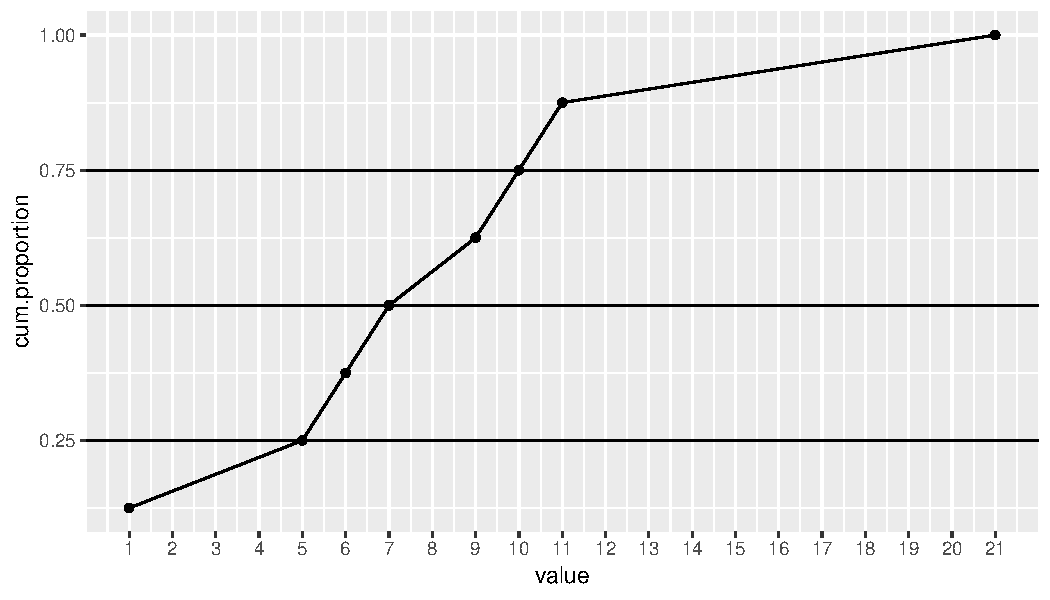
\includegraphics[width=\maxwidth]{figure/quartile_1-1} 

}

\caption[Cumulative proportions]{Cumulative proportions.}\label{fig:quartile_1}
\end{figure}



The graphical way is far easier for large data sets. If we plot the cumulative proportions for the ages of the 1000 children, we obtain Figure \ref{fig:quartile_2}. We see a nice S-shaped curve. We also see that the three horizontal quartile lines no longer intersect the curve at specific values, so we need a rule to determine what value to pick. By eyeballing we can find that the first quartile is somewhere between 4 and 5. This tell us that the youngest 25\% of children have ages of 5 or less\footnote{If you don't see that, read again the section on cumulative proportions and how they are computed.}. The second quartile is somewhere between 6 an 7, so we know that 50\% of the youngest children is 7 years old or younger The third quartile is somewhere between 8 and 9 and this tells us that the youngest 75\% of the children is age 9 or younger Thus, we can call 5, 7 and 9 our three quartiles.



\begin{figure}

{\centering 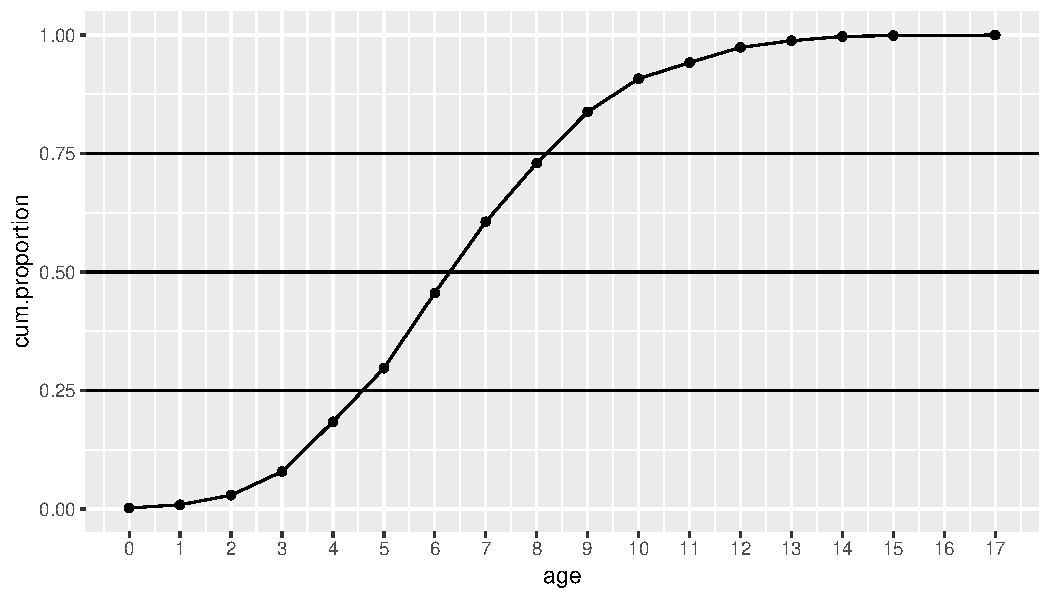
\includegraphics[width=\maxwidth]{figure/quartile_2-1} 

}

\caption[Cumulative proportions]{Cumulative proportions.}\label{fig:quartile_2}
\end{figure}




Alternatively, we could also use the frequency table (Table \ref{tab:frequency_1}). First, if we want to have 25\% of the children that are the youngest, and we know that we have 1000 children in total, we should have $0.25 * 1000=250$ children in the first group. So if were to put all the children in a row, ordered from youngest to oldest, we want to know the age of the 250th child.

In order to find the age of this 250th child, and we look at Table \ref{tab:frequency_1}, we see that 29.7 \% of the children have an age of 5 or less (297 children), and 18.4 \% of the children have an age of 4 or less (184 children). This tells us that the 250th child must be 5 years old. Furthermore, if we want to find a cut-off age for the oldest 25\%, we see from the table, that 83.8\% of the children (838 children) have an age of 9 or less, and 73.0\% of the children (730) have an age of 8 or less. Therefore, the age of the 750th child (when ordered from youngest to oldest) must be 9.


What we just did for quartiles, (i.e. 0.25, .50, 0.75) we can do for any proportion between 0 and 1. We then no longer call them quartiles, but \textit{quantiles}. A quantile is the value below which a given proportion of observations in a group of observations fall. From this table it is easy to see that a proportion of 0.606 of the children have an age of 7 or less. Thus, the 0.606 quantile is 7. One often also sees \textit{percentiles}. Percentiles are very much like quantiles, except that they refer to percentages rather than proportions. Thus, the 20th percentile is the same as the 0.20 quantile. And the 0.81 quantile is the same as the 81st percentile.



\subsection{Exercises}

% latex table generated in R 3.5.0 by xtable 1.8-2 package
% Tue Aug 28 11:36:32 2018
\begin{table}[ht]
\centering
\caption{Freqency table for x, with proportions and cumulative proportions.} 
\label{tab:frequency_2}
\begin{tabular}{rrrr}
  \hline
x & frequency & proportion & cum.proportion \\ 
  \hline
   0 &    6 & 0.030 & 0.030 \\ 
     1 &   25 & 0.125 & 0.155 \\ 
     2 &   55 & 0.275 & 0.430 \\ 
     3 &   44 & 0.220 & 0.650 \\ 
     4 &   36 & 0.180 & 0.830 \\ 
     5 &   20 & 0.100 & 0.930 \\ 
     6 &    9 & 0.045 & 0.975 \\ 
     7 &    4 & 0.020 & 0.995 \\ 
     8 &    1 & 0.005 & 1.000 \\ 
   \hline
\end{tabular}
\end{table}


\begin{enumerate}
\item Look at Table \ref{tab:frequency_2}. Determine the 10th quantile for variable \textbf{x}.

\item Determine the 95th percentile.

\item Determine the first quartile.

\item Determine the second quartile.

\item Determine the 50th percentile.

\item Determine the third quantile.

\item Determine the 0.75 quantile.

\item Suppose we have the values {6,5,4,8,6,5,6,4,5,6,7,8}. Determine the third quartile.

\item Suppose we have the values {4,4,4,8,6,4,6,4,5,6,7,8,9}. Determine the third quartile.

\item From Figure \ref{fig:quartile_3}, determine the 30th, 40th and 90th percentiles.

\begin{figure}

{\centering 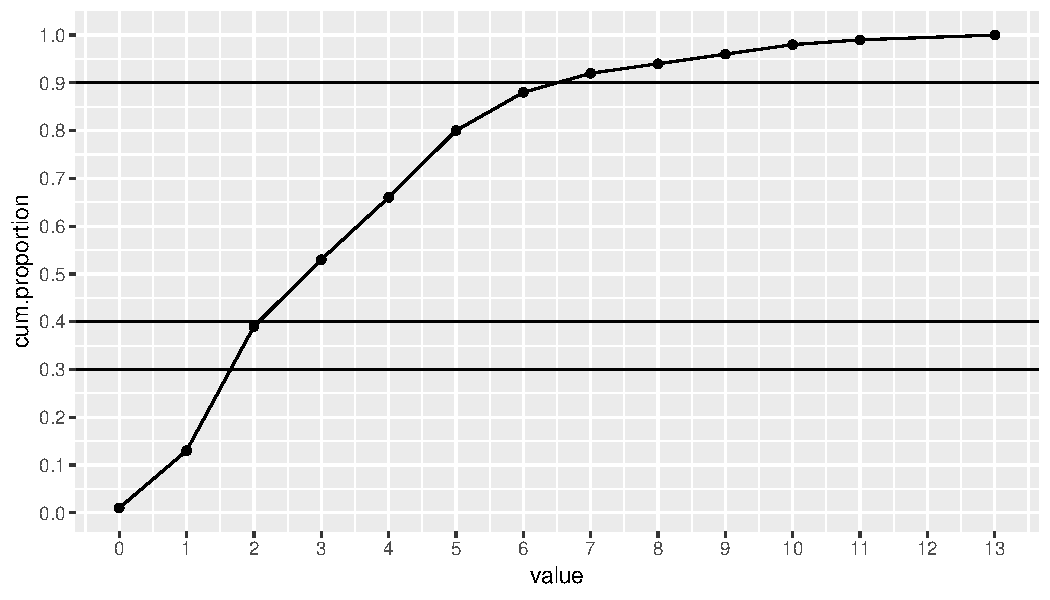
\includegraphics[width=\maxwidth]{figure/quartile_3-1} 

}

\caption[Cumulative proportions]{Cumulative proportions.}\label{fig:quartile_3}
\end{figure}



\item Yesterday you did an IQ test, together with 999 other students. Today you here that you scored 100 points. They tell you that the 8th percentile was a score of 80, and the 9th percentile was a score of 100. What does that tell you about your performance yesterday?


\end{enumerate}






\section{Mean, median and mode}

\subsection{The mean}
The mean of set of values is the same as the average. Suppose we have the values 1, 2 and 3, then we compute the mean (or average) by first adding these numbers and then divide them by the number of values we have. In this case we have three values, so the mean is equal to $(1 + 2 + 3)/3 = 2$. In statistical formulas, the mean is indicated by a bar above the variable. So if our values of variable $y$ are 1, 2 and 3, then we denote the mean by $\bar{y}$ (pronounced as y-bar). For taking the sum of a set of values, statistical formulas show a $\Sigma$ (pronounced as sigma). So we often see the following formula for the mean of a set of $n$ values for variable $y$:

\begin{equation}
\bar{y} = \frac{\Sigma_i^n y_i}{n}
\end{equation}

In words, we take every value for $y$ from 1 to $n$ and sum them, and the result is divided by $n$.

If we take another example, suppose we have variable $x$ with the values {6, -3, and 21}, then the mean of $x$, $\bar{x}$, equals:

\begin{equation}
\bar{x} = \frac{x_1 + x_2 + x_3}{n} = \frac{6 + (-3) + 21}{3} = \frac{24}{3} = 8
\end{equation}



\subsection{The median}
The mean is a measure of central tendency: if the mean is 100, it means the values tend to cluster around this value. A different measure of central tendency is the median. The median is nothing but the middle value. Suppose we have the values 45, 567, and 23. Then what value lies in the middle? Let's first order them from small to large to get a better look, then we get 23, 45 and 567. Then the value in the middle is of course 45.

Suppose we have the values 45, 45, 45, 65, and 23. What is the middle value? We first order them again and see what is in the middle: 23, 45, 45, 45 and 65. Obviously now 45 is the median. You can also see that half of the values is smaller than this value, and half of the values is larger than this value. The median therefore is the same as the second quartile.

What if we have two values in the middle? Suppose we have the values 46, 56, 45 and 34. If we order them we get 34, 45, 46 and 56. Now there are two values in the middle: 45 and 46. In that case, we take the average of these two middle values, so the median is 45.5. For quantitative variables that have a more more or less symmetric distribution, the mean is best used. For quantitative variables that don't have a symmetric distribution, it is usually more informative to use the median. An example of such a situation is income. Figure \ref{fig:median} shows a typical distribution of incomes per country. The distribution is highly asymmetric, it is severely skewed to the right. The bulk of the values are between 20,000 and 40,000, with only a very few extreme values. Even though there are only a few people with a very extreme income, the extreme income values have a huge effect on the mean.

\begin{figure}

{\centering 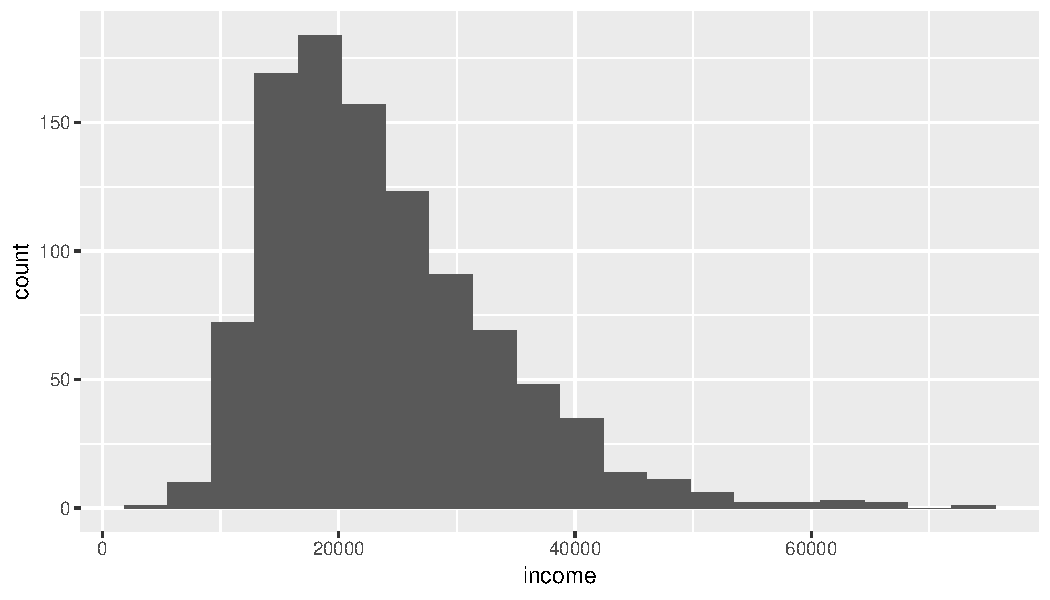
\includegraphics[width=\maxwidth]{figure/median-1} 

}

\caption[Distribution of yearly income]{Distribution of yearly income.}\label{fig:median}
\end{figure}



The mean of the distribution turns out to be \ensuremath{2.3604\times 10^{4}}. The largest value in the distribution is an income of \ensuremath{7.5051\times 10^{4}}.

[1] 1


If we would change this value into 99561, you see an immediate impact on the mean: the mean is then \ensuremath{2.3594\times 10^{4}}. This means that the mean is very sensitive to extreme values. Very small changes in a data set can have huge effects. The median on the other hand is much more stable. The median remains unaffected by slight changes in the extremes. This because it only looks at the value below which 50\% of the values are. That value is unaffected by a change in the most extreme values, as long as the order of the values remains the same.




\subsection{The mode}
A third measure of central tendency is the \textit{mode}. The mode is defined as the value that we see most frequently in a series of values. For example, if we have the series 4, 7, 5, 5, 6, 6, 6, 4, then the value observed most often is 6 (three times). Modes are easily inferred from frequency tables: the value with the largest frequency is the mode.

The mode can also be determined for categorical variables. If we have the observed values "Dutch", "Danish", "Dutch", and "Chinese", the mode is "Dutch" because that is the value that is most often observed.

If we look back at the distribution in Figure \ref{fig:median}, we see that the peak of the distribution is around the value of 19,000. However, if this is the mode, we cannot say. Because income is a more or less continuous variable, every value observed in the Figure occurs only once: there is no value of income with a frequency more than 1. So technically, there is no mode. However, if we split the values into 20 bins, like we did for the histogram in Figure \ref{fig:median}, we see that the fifth bin has the highest frequency. In this bin there are values between 17000 and 21000, so our mode could be around there. If we really want a value, we could decide to taken the average value in the fifth bin. There are many other statistical tricks to find a value for the mode, where technically there is none. The point is that for the mode, we're looking for the value or the range of values that are most frequent. Graphically, it is the value under the peak of the distribution. Similar to the median, the mode is also quite stable: it is not much affected by extreme values and is therefore to be preferred over the mean in the case of assymetric distributions.



\subsection{Exercises}

\begin{enumerate}

\item If we have values 56, 78, 23 and 45, what is the mean?

\item If we have values 56, 78, 23 and 45, what is the median?

\item If we have values 56, 23, 78, 23 and 45, what is the mode?

\item Figure \ref{fig:mode} shows a distribution of systolic bloodpressure measures in older men. What would be more or less the mode of these values?

\begin{figure}

{\centering 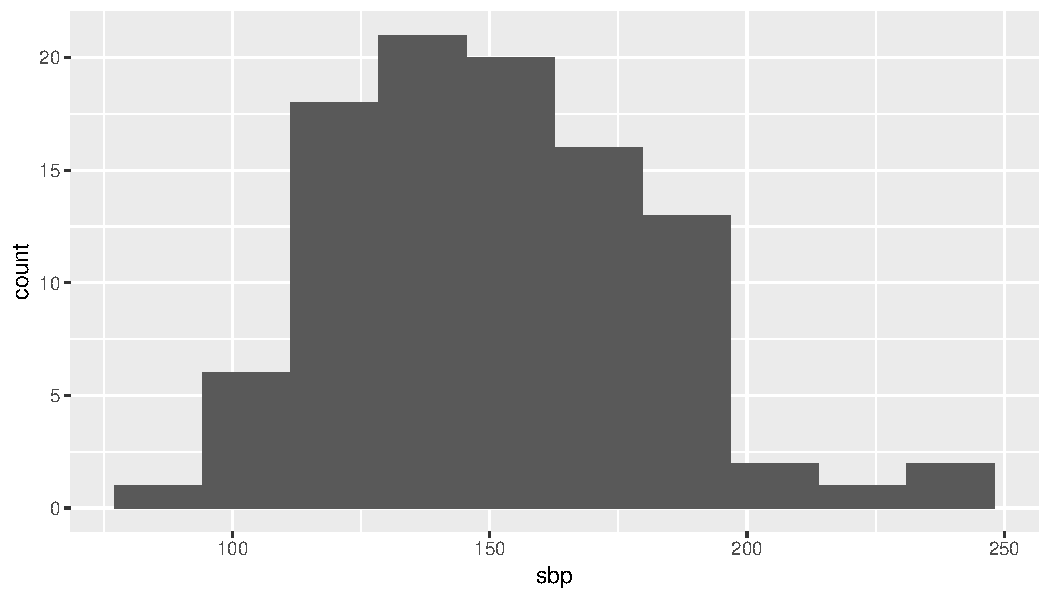
\includegraphics[width=\maxwidth]{figure/mode-1} 

}

\caption[Distribution of systolic bloodpressure]{Distribution of systolic bloodpressure.}\label{fig:mode}
\end{figure}



\item Figure \ref{fig:<quartile_3} shows a distribution of values. What would be more or less the median of these values?

\item Figure \ref{fig:mode_2} shows a distribution of number of bicycles for 100 households. If you could choose only one statistic to describe this distribution, what would you choose to report: the mean, the mode or the median? Motivate your answer.

\begin{figure}

{\centering 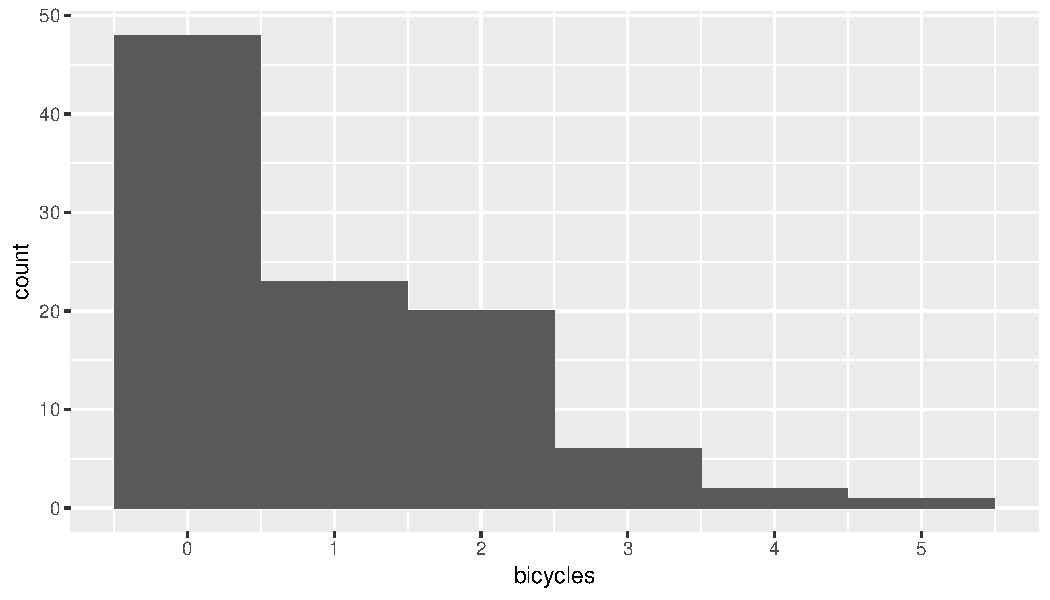
\includegraphics[width=\maxwidth]{figure/mode2-1} 

}

\caption[Distribution of systolic bloodpressure]{Distribution of systolic bloodpressure.}\label{fig:mode2}
\end{figure}





\end{enumerate}


% \section{Relationship between measures of tendency and measurement level}
% 
% There is a close relationship between measures of tendency and measurement level. For numeric variables, all three measures of tendency are meaningfull. Suppose you have the numeric variable age measured in years, with the values 56, 68, 68, 99 and 100. Then it is meaningful to say that the average age is 78.2 years, that the median age is 68 years, and that the mode is 68 years. 
% 
% For ordinal variables, it is quite different. Suppose you have 5 T-shirts, with the following sizes: M, S, M, L, XL. Then what is the average size? There are no numeric values here to put in the algebraic formula. But we can determine the median: if we order the values from small to large we get the set S, M, M, L, XL and we see that the middle value is M. So M is our median in this case. \footnote{However, suppose that our collection of T-shirts had the following sizes: S, M, L, L. Then there would be no single middle value in we would have to average the M and L values, which would be impossible!} The other meaningful of tendency for ordinal variables is the mode. 
% 
% For categorical variables, both the mean and the median are pointless to report. Suppose we have the nominal variable Study Programme with observed values "Medicine", "Engineering", "Engineering", "Mathematics", and "Biology". It would be impossible to derive a numerical mean, nor would it be possible to determine the middle value to determine the median, as there is no logical or natural order (unless you see one?). It is meaningful though to report a mode. It would be meaningful to state that the study programme mentioned most often in the news is "Psychology", or that the most popular study program in India is "Engineering". Thus, for categorical variables, both dichotomous and nominal variables, only the mode is a meaningful measure of central tendency.
% 
% As stated earlier, the appearance of a variable in a data matrix can be quite misleading. Categorical variables and ordinal variables can often look like numeric variables, which makes it very tempting to compute means and medians where they are completely meaningless. Take a look at Table \ref{tab:modemedian}. It is entirely possible to compute the average University, Size, or Programme, but it would be utterly senseless to report these values. 
% 
% It is entirely possible to compute the median University, Size, or Programme, but it is only meaningful to report the median for the variable Size, as Size is an ordinal value. Reporting that the median size is equal to 2 is saying that about half of the study programs is of medium size or small, and about half of the study programs is of medium size or large. 
% 
% It is entirely possible to compute the mode for the variables University, Size, or Programme, and it is always meaningful to report them. It is meaningful to say that in your data there is no University that is observed more than others. It is meaningful to report that most study programmes are of medium size, and that most study programmes are study programme number 2 (don't forget to look up and write down which study programme that actually is!).
% 
% 
% 
% <<tab_modemedian, fig.height=4, echo=FALSE, fig.align='center', fig.cap='A frequency table of nationalities.', results='asis' >>=
% set.seed(123)
% University <- c(1,2,3,4,5,6) 
% Size <- c(1,3,2,2,3,2)
% Programme <- c(2,2,3,3,4,1)
% data_frame(University, Size, Programme) %>% 
%         xtable(caption="Study programs and their relative sizes (1=small, 2=medium, 3=large) for six different universities.", label="tab:modemedian", digits=0  ) %>%
%         print(include.rownames=F, caption.placement = "top")
% @
% 
% 
% 
% 
% \section{Variation}
% 
% Suppose we measure the height of 3 children and their heights (in cms) are rep(120,3). There is no variation in height: all heights are the same. There are no differences. Then the average height is 120, the median height is 120, and the mode is 120. 
% 
% Now suppose their heigths are set.seed(1234);round(runif(3,119,120), 0). Now there are differences: one child is smaller than the other two, who have the same height. There is some variation now. We know how to quantify the mean, which is set.seed(1234);mean(round(runif(3,119,120), 0)), we know how to quantify the median, which is 120, and we know how to quantify the mode, which is also 120. But how do we quantify the variation? Is there a lot of variation, or just a little, and how do we measure it? 
% 
% One way you could think of is measuring the distance between the lowest value and the highest value. This we call the \textit{range}. The lowest value is 119, and the highest value is 120, so the range of the data is equal to $120-119=1$. As another example, suppose we have the values 20, 20, 21, 20, 19, 20 and 454. Then the range is equal to $454-19=435$. That's a large range, for a series of values that for the most part hardly differ from another. 
% 
% Instead of measuring the distance from the lowest to the highest value, we could also measure the distance between the first and the third quartile. This distance is called the \textit{interquartile distance}. Suppose that we have a large number of systolic bloodpressure measurements, where 25\% are 120 or lower, and 75\% are 147 or lower, then the interquartile distance is equal to $147-120=27$. 
% 
% Another measure for spread is \textit{variance}, and variance is based on the \textit{sum of squares}. 
% 
% \subsection{Sum of squares}
% 
% What we call a sum of squares is actually a sum of squared deviations. But deviations from what? First we have to know whether we are interested in the variation around what value. For instance we could be interested in how far the values set.seed(1234);round(runif(3,119,120), 0) deviate from 0. The first differs 119, and the second and third differ 120. All values differ in a positive sense from 0: all values are positive. The deviations from zero are then 119, 120 and 120. Squaring these, we get the squared deviations, $119^2$, $120^2$ and $120^2$ so $14161$, $ 14400$ and $ 14400$. Adding these squared deviations, we obtain 42961 as the sum of squares. A sum of squares that uses deviations from zero is called the \textit{total sum of squares}.
% 
% We could also be interested in how much the values set.seed(1234);round(runif(3,119,120), 0) vary around the \textit{mean} of these values. The mean of these three values equals set.seed(1234);mean(round(runif(3,119,120), 0)). The first value differs $119-set.seed(1234);mean(round(runif(3,119,120), 0))= set.seed(1234);119-mean(round(runif(3,119,120), 0))$, the second value differs $120-set.seed(1234);mean(round(runif(3,119,120), 0))= set.seed(1234);120-mean(round(runif(3,119,120), 0))$, and the third value also differs $120-set.seed(1234);mean(round(runif(3,119,120), 0))= set.seed(1234);120-mean(round(runif(3,119,120), 0))$.
% 
% Always when we look at deviations from the mean, some deviations are positive and some deviations will be negative (except when there is no variation). If we want to measure variation, it should not matter whether deviations are positive or negative: any deviation should add to the total variation in a positive way. Moreover, if we would add up all deviations from the mean, we would always end up with 0. So that is why we should better make all deviations positive, and this can be done by taking the square of the deviations. So for our three values 119, 120 and 120, we get the deviations -0.67, +0.33 and +0.33, and if we square these deviations, we get $(-0.67)^2$, $(+0.33)^2$ and $(+0.33)^2$, so -0.67^2, 0.33^2 and 0.33^2. If we add these three squares, we obtain the sum $(-0.67)^2+0.33^2+0.33^2=-0.67^2+0.33^2+0.33^2$.   
% 
% In most cases, the sum of squares (SS) refers to the sum of squared deviations from the mean. In brief, suppose you have $n$ values of a variable $y$, you first take the mean of those values (this is $\bar{y}$), you subtract this mean from each of these $n$ values ($y-\bar{y}$), then you take the squares of these deviations ($(y-\bar{y})^2$), and then add them toghether (take the sum of these squared deviations, $\Sigma (y-\bar{y})^2)$. In formula form, this process looks like:
% 
% \begin{equation}
% SS = \Sigma_i^n (y_i-\bar{y})^2
% \end{equation}
% 
% As an example, suppose you have the values 10, 11 and 12, then the average value is 11. Then the deviations from the mean are -1, 0 and 1. If you square them you get 1, 0 and 1, and if you add these three values, you get $SS=2$. In formula form:
% 
% 
% \begin{equation}
% SS = (y_1-\bar{y})^2 + (y_2-\bar{y})^2 (y_3-\bar{y})^2 = (10-11)^2 + (11-11)^2 (12-11)^2= (-1)^2 + 0^2 + 1^2=2
% \end{equation}
% 
% Now let's use some values that are more different from eachother, but with the same mean. Suppose you have the values 9, 11 and 13. The average value is still 11, but the deviations from the mean are larger. The deviations from 11 are -2. 0 and +2. Taking the squares, you get 4, 0 and 4 and if you add them you get $SS=8$.
% 
% \begin{equation}
% SS = (y_1-\bar{y})^2 + (y_2-\bar{y})^2 (y_3-\bar{y})^2 = (9-11)^2 + (11-11)^2 (13-11)^2= (-2)^2 + 0^2 + 2^2=8
% \end{equation}
% 
% Thus, the more values differ from eachother, the larger the deviations from the mean. And the larger the deviations from the mean, the larger the sum of squares. The sum of squares is therefore a nice measure of how much values differ from eachother.
% 
% \subsection{Variance and standard deviation}
% 
% The sum of squares can be seen as some kind of total variation: all deviations from a certain value are added up. This means that the more data values you have, the larger the sums of squares. Oftentimes, you are not interested in the total variation, but you're interesed in the average variation: how much does the avarage value differ from the mean? Suppose we have the values 10, 11 and 24. The mean is then $45/3=15$. We have two values that are smaller than the average and one value that is larger than the average, so two negative deviations and one positive deviation. Squaring them makes them all positive. The squared deviations are 25, 16, and 81. The third value has a huge squared deviation (81) compared to the other two values. If we take the \textit{average} squared deviation, we get $(25+16+81)/3= (25+16+81)/3$. So the average squared deviation is equal to (25+16+81)/3. This value we call the \textit{variance}. So the variance of a bunch of values is nothing but the $SS$ divided by the number of values, $n$. The variance is \textit{the average squared deviation from the mean}. The symbol used for the variance is usually $\sigma^2$ (pronounced as "sigma squared").
% 
% \begin{equation}
% \sigma^2 = \frac{SS}{n}= \frac{\Sigma_i^n (y_i-\bar{y})}{n}
% \end{equation}
% 
% 
% As an example, suppose you have the values 10, 11 and 12, then the average value is 11. Then the deviations are -1, 0 and 1. If you square them you get 1, 0 and 1, and if you add these three values, you get $SS=2$. If you divide this by 3, you get the variance: 0.67. Put differently, if the squared deviations are 1, 0 and 1, then the average squared deviation (i.e., the variance) is $\frac{1+0+1}{3}=0.67$.
% 
% As another example, suppose you have the values 8, 10, 10 and 12, then the average value is 10. Then the deviations from 10 are -2, 0, 0 and +2. Taking the squares, you get 4, 0, 0 and 4 and if you add them you get $SS=8$. To get the variance, you divide this by 4: $8/4=2$. Put differently, if the squared deviations are 4, 0, 0 and 4, then the average squared deviation (i.e., the variance) is $\frac{4+0+0+4}{4}=2$.
% 
% Often we also see another measure of variation: the \textit{standard deviation}. The standard deviation is the root of the variance and is therefore denoted as $\sigma$:
% 
% \begin{equation}
% \sigma = \sqrt{\sigma^2}=\sqrt{  \frac{\Sigma_i^n (y_i-\bar{y})}{n}}
% \end{equation}
% 
% 
% \subsection{Exercises}
% 
% \begin{enumerate}
% \item Suppose we have the values 9, 6, 5, and 66. What is the range?
% \item Suppose we have the values -9, 6, -5, and 66. What is the range?
% \item Suppose we have the values 9, 6, 5, and 4. What is the sum of squared deviations from 0?
% \item Suppose we have the values 9, 6, 5, and 4. What is the sum of squared deviations from the mean?
% \item Suppose we have the values -7, 6, -5, and 6. What is the sum of squared deviations from the mean?
% \item Suppose we have the values -7, 6, -5, and 6. What is the variance?
% \item Suppose we have the values 77, 76, and 78. What is the standard deviation?
% \end{enumerate}
% 
% Answers:
% 
% 
% \begin{enumerate}
% \item Smallest value is 5, largest value is 66. The range is $66-5=61$.
% \item Smallest value is -9, largest value is 66. The range is $66-(-9)=75$.
% \item $9^2+6^2+5^2+4^2=81+36+25+16=81+36+25+16$
% \item The mean is $(9+6+5+4)/4=(9+6+5+4)/4$. So we have $(9-6)^2+(6-6)^2+(5-6)^2+(4-6)^2=9+0+1+4=14$.
% \item The mean is $(-7+6-5+6)/4=(-7+6-5+6)/4$. So we have $(-7)^2+6^2+(-5)^2+6^2=49+36+25+36=49+36+25+36$.
% \item The mean is 0. So the sums of squares equals $(-7)^2+6^2+(-5)^2+6^2=49+36+25+36=49+36+25+36$. Then the variance is $49+36+25+36/4=(49+36+25+36)/4$.
% \item The average is $(77+76+78)/3=77$. The sum of squares is then $(-1)^2+0^2+1^2=2$. The variance is then $2/3=0.67$. The standard deviation is the root of the variance, so $\sqrt{0.67}=round(sqrt(0.67),2)$.
% \end{enumerate}
% 
% \section{Distributions}
% 
% 
% <<distr_1, fig.height=4, echo=FALSE, fig.align='center', message=F, fig.cap='A frequency distribution' >>=
% set.seed(123)
% numbers <- runif(20, 1,10) %>%  round(0)
% data.frame(numbers) %>% 
%         ggplot(aes(numbers)) + geom_histogram(binwidth = 1, bins=10)  +
%         xlab('observed values') + ylab('count')+
%         scale_x_continuous(breaks=seq(1,10))
% @
% 
% Variables have distributions. That means that if you put all the values you observed in order from low to high, you see a certain shape. For example, take the set of following numbers: numbers. If you plot these values on the horizontal axis, and how often they are observed (the \textit{frequency} or \textit{count}) on the vertical you get the frequency plot in Figure \ref{fig:distr_1}. Such a frequency plot is referred to as a \textit{bar chart}.
% 
% Often a \textit{histogram} is plotted. A histogram is very much like a frequency plot or bar chart, except that groups of values can be taken together. Such a group of values is called a \textit{bin}. Figure \ref{fig:distr_2} shows the same data, but uses only 5 bins: for the first bin, we take values of 1 and 2, for the second bin we take values 3 and 4 together, etcetera, until we take vales 9 and 10 for the fifth bin. For each bin, we compute how often we observe the values in that bin. Histograms are also for continous data, for instance if we have values like 3.4, 2,1, etcetera. All values within a bin are defined by their rounded value. For instance, in Figure \ref{fig:distr_2}, all possible values between 2.5 and 4.5 will end up in the second bin. The \textit{binwidth} is here 2: all values between 2.5 and 4.5 are taken to lie in the second bin, and the distance between these values is $4.5-2.5=2$. 
% 
% <<distr_2, fig.height=4, echo=FALSE, fig.align='center', warning=FALSE, message=F, fig.cap='A histogram' >>=
%  data.frame(numbers ) %>% 
%         ggplot(aes(numbers)) + geom_histogram(binwidth = 2, center=1.5)  +
%         xlab('observed values') + ylab('count') +
%         scale_x_continuous(breaks=seq(1, 10))
% @
% 
% 
% Histograms can be rather coarse-looking. A more elegant representation of how the frequency of certain values is distributed across a continuum is a \textit{density plot}. Density plots are particularly suited for large amounts of non-discrete values, typically more than 1000. Figure \ref{fig:distr_3} shows a density plot of 1000 temperature values between 50 and 60 Fahrenheit, where all values had a precision of 4 decimal points (i.e., values like 53.9845, 56.0912, etc.). The plot suggests that values around 55 degrees are most frequent, and that values around 52 or around 58 are rather infrequent in the data set. On the vertical axis, we no longer see count or frequency, but we see density. Density is defined such that the area under the curve equals 1. Density plots are for large data sets, so in the particular counts we are no longer interested: we're more interested in relative frequencies: how often are certain values observed, relative to other values. From this density plot, it is very clear that relatively speaking there are more values between 54 and 55 than between 52 and 53. 
%  
% <<distr_3, fig.height=4, echo=FALSE, fig.align='center', message=F,warning=FALSE, fig.cap='Density plot of 1000 observed temperature measures.' >>=
% set.seed(1234) 
%  data_frame(temperature = rnorm(1000,55, 1)) %>% 
%         ggplot(aes(temperature)) + geom_density()  +
%         scale_x_continuous(breaks=seq(50, 60)) +
%         xlim(c(50,60))
% @
% 
% 
% 
% 
% \subsection{The normal distribution}
% 
% Sometimes histograms and density plots of observed variables bear close resemblance to \textit{theoretical} distributions. For instance, Figure \ref{fig:distr_3} bears close resemblance to the theoretical \textit{normal} distribution with mean 5 and standard deviation 1. That density is plotted in Figure \ref{fig:distr_4}. Because of its bell-shaped form, the normal distribution is sometimes informally called 'the bell curve'. 
% 
% 
% <<distr_4, fig.height=4, echo=FALSE, fig.align='center', warning=FALSE, fig.cap='The theoretical normal distribution.' >>=
% shaded<-  data_frame(x = seq(54, 56,0.1),  y = dnorm(seq(54, 56,0.1), 55, 1))
% shadedleft <-  data_frame(x=seq(50, 55-1.96 ,.1),y= dnorm(seq(50, 55-1.96 ,.1), 55, 1))
% shadedright <-  data_frame(x=seq(55+1.96 , 60,  .1),y= dnorm(x=seq(55+1.96 , 60,  .1), 55, 1))
%   data_frame(temperature = seq(50,60,0.1)) %>% 
%         ggplot()+ 
%         geom_line(aes(x=temperature, y = dnorm(temperature, mean=55, sd=1))) + 
%         scale_x_continuous(breaks=seq(50, 60))+
%         geom_area(data=shaded, mapping=aes(x=seq(54,56,.1),y= dnorm(seq(54,56,.1), 55, 1)   ), alpha=0.5)+
%         geom_area(data=shadedleft, mapping=aes(x=seq(50 , 55-1.96,  .1),y= dnorm(x=seq(50 , 55-1.96,  .1), 55, 1) ), alpha=0.5)+
%         geom_area(data=shadedright, mapping=aes(x=seq(55+1.96 , 60,  .1),y= dnorm(x=seq(55+1.96 , 60,  .1), 55, 1) ), alpha=0.5)+
%         ylab("density") +
%           geom_text(x=55, y=0.2, label="68 percent")+
%           geom_text(x=52, y=0.05, label="2.5 percent")+
%           geom_text(x=58, y=0.05, label="2.5 percent")
% @
% 
% They look so similar, that it could well be that if we would have had more than 1000 temperature measures, say 100 million measures, the density plots of the observed temperature measures would be indistinguishable from the theoretical normal distribution. 
% 
% Mathematicians have discovered many interesting things about the normal distribution. If a variable closely resembles a normal distribution, you can infer many things. One thing we know about the normal distribution is that the mean, mode and median are always the same. Another thing we know from theory is that the inflection points\footnote{The inflection point is where concave turns into convex, and vice versa. Mathematically, the inflection point can be found by equating the second derivative of a function to 0.} are one standard deviation away from the mean.  Figure \ref{fig:distr_4} shows the two inflection points. From theory we also know that if a variable has a normal distribution, 68\% of the observed values lies between these two inflection points. We also know that 5\% of the observed values lies more than 1.96 standard deviations away from the mean (2.5\% on both sides). Theorists have constructed tables that make it easy to see what proportion of values lies more than $1, 1.1, 1.2 \dots, 3.8, 3.9, \dots$ standard deviations away from the mean. These tables are easy to find online or in books, and these are fully integrated into statistical software like SPSS and R. Because all these percentages are known for the number of standard deviations, it is easier to talk about the \textit{standard normal distribution}. 
% 
% In such tables, you find information only about the \textit{standard normal distribution}. The standard normal distribution is a normal distribution where all scores have been \textit{standardized}. Standardized means that the the scores have an average of 0 and a standard deviation of 1. Such standardized scores are obtained if you subtract the mean score from each score, and divide the result by the standard deviation. A standardized score is often denoted as a $Z$-score. Thus in formula form, a normally distributed score $x$ is standardized by using the following equation:
% 
% 
% \begin{equation}
% Z = \frac{x - \bar{x}}{\sigma}
% \end{equation}
% 
% 
% 
% <<normal_1, fig.height=4, echo=FALSE, fig.align='center', fig.cap='A frequency table of nationalities.', results='asis' >>=
% set.seed(123)
% x <- rnorm(10, 10, 5) %>% round(1)
% Z <- scale(x)[1:10,1]
% data_frame(x, Z) %>% 
%         xtable(caption="Standardizing scores.", label="tab:normal_1", digits=1   ) %>%
%         print(include.rownames=F, caption.placement = "top")
% @
% 
% Table \ref{tab:normal_1} shows an example set of $x$-values that are standardized. The average of the $x$-values turns out to be 10.38, and the standard deviation 4.77. By subtracting the mean, we make all $Z$-scores be on average 0, and by dividing by the standard deviation, the standard deviation of the $Z$-scores becomes 1. 
% 
% This standardization makes it much easier to look up certain facts about normal distribution. For instance, if we go back to the normally distributed temperature values, we see that the average is 55 degrees, and the standard deviation is 1. Thus, if we take all temperature values, subtract 55 and divide by 1, we get standardized temperatures with average 0 and standard deviation 1. The result is shown in Figure \ref{fig:normal_2}. We know that the inflection point lies at one standard deviation below and above the mean. The mean is 55, and the standard deviation equals 1, so the inflection points are at $55-1=54$ and $55+1=56$. Thus we know that 68\% of the values are between 54 and 56. 
% 
% 
% <<normal_2, fig.height=4, echo=FALSE, fig.align='center', warning=FALSE, fig.cap='The theoretical normal distribution.' >>=
% shaded<-  data_frame(x = seq(-1, 1,0.1),  y = dnorm(seq(-1, 1,0.1), 0, 1))
% shadedleft <-  data_frame(x=seq(-5, 0-1.96 ,.1),y= dnorm(seq(-5, 0-1.96 ,.1), 0, 1))
% shadedright <-  data_frame(x=seq(0+1.96 , 5,  .1),y= dnorm(x=seq(0+1.96 , 5,  .1), 0, 1))
%   data_frame(temperature = seq(-5,5,0.1)) %>% 
%         ggplot()+ 
%         geom_line(aes(x=temperature, y = dnorm(temperature, mean=0, sd=1))) + 
%         scale_x_continuous(breaks=seq(-5, 5))+
%         geom_area(data=shaded, mapping=aes(x=seq(-1,1,.1),y= dnorm(seq(-1,1,.1), 0, 1)   ), alpha=0.5)+
%         geom_area(data=shadedleft, mapping=aes(x=seq(-5 , 0-1.96,  .1),y= dnorm(x=seq(-5 , 0-1.96,  .1), 0, 1) ), alpha=0.5)+
%         geom_area(data=shadedright, mapping=aes(x=seq(0+1.96 , 5,  .1),y= dnorm(x=seq(0+1.96 , 5,  .1), 0, 1) ), alpha=0.5)+
%         ylab("density") +
%           geom_text(x=0, y=0.2, label="68 percent")+
%           geom_text(x=-3.5, y=0.05, label="2.5 percent")+
%           geom_text(x=3.5, y=0.05, label="2.5 percent")
% @
% 
% How do we know that 68\% of the observations lie between the two inflection points? Similar to proportions and cumulative proportions, we can plot the cumulative normal distribution. Figure \ref{fig:normal_3} shows the cumulative proportions curve for the normal distribution. Note that we no longer see dots because the variable z is continuous.
% 
% <<normal_3, fig.height=4, echo=FALSE, fig.align='center', warning=FALSE, fig.cap='The cumulative standard normal distribution.' >>=
%   data_frame(z = seq(-5,5,0.1)) %>% 
%           mutate(cum.prob= pnorm(z)) %>% 
%         ggplot(aes(x=z, y=cum.prob) ) + 
%         geom_line() +
%         scale_x_continuous(breaks=seq(-6, 6)) +
%           geom_segment(x=-4.9,y=pnorm(-1),xend=-1, yend=pnorm(-1), linetype="dashed")+
%           geom_segment(x=-4.9,y=pnorm(1),xend=1, yend=pnorm(1), linetype="dashed")+
%           geom_segment(x=-1,y=0,xend=-1, yend=pnorm(-1), linetype="dashed")+
%           geom_segment(x=1,y=0,xend=1, yend=pnorm(1), linetype="dashed") + 
%           geom_text(aes(x=-5.8,pnorm(-1)),label=paste(round(pnorm(-1),2)))+
%           geom_text(aes(x=-5.8,pnorm(1)),label=paste(round(pnorm(1),2)))
% @
% 
% We know that the two inflection points lie one standard deviation below and above the mean. Thus, if we look at a $z$-values of 1, we see that the cumulative probability equals about pnorm(1). This means that pnorm(1)*100 \% of the $z$-values are lower than 1. If we look at a $z$-values of -1, we see that the cumulative probability equals about pnorm(-1). This means that pnorm(-1)*100 \% of the $z$-values are lower than -1. Therefore, if we want to know what percentage of the $z$-values lie between -1 and 1, we can calculate this by subtracting pnorm(-1) from pnorm(1), which equals pnorm(1)-pnorm(-1), which corresponds to slightly over 68\%.
% 
% All quantiles for the standard normal distribution can be looked up online\footnote{see for example ....} or in books. Table \ref{tab:normal_4} gives a short list of quantiles. From this table, you see that 1\% of the $z$-values is lower than -2.33, and that 25\% of the $z$-values is lower than -0.67. We also see that half of all the $z$-values is lower than 0.00 and that 10\% of the $z$-values is larger than 1.28, and that the 1\% largest values are higher than 2.33.
% 
% <<normal_4, fig.height=4, echo=FALSE, fig.align='center', fig.cap='A frequency distribution', results='asis' >>=
% proportion <- c(0.01, 0.10, 0.25, 0.50, 0.75, 0.90, 0.99)
% z <- qnorm(proportion)  
% data.frame(cum.proportion=proportion, z) %>%
%         xtable(caption="Some quantiles for the standard normal distribution.", label="tab:normal_4", digits=2   ) %>%
%         print(include.rownames=F, caption.placement = "top")
%         
% @
% 
% 
% Thus, if we return to our temperatures with mean 55 and standard deviation, we know from Table \ref{tab:normal_4} that 99\% of the temperatures are below 55 + 2.33 times the standard deviation=  $55+2.33*1$=55+2.33*1 degrees. 
% 
% As an other example. Suppose we have IQ scores that are normally distributed with a mean of 100 and a standard deviation of 15. What IQ score would be the 90th percentile? From Table \ref{tab:normal_4} we see that the 90th percentile is a $z$-value of round(qnorm(0.90),2). Thus,the 90th percentile for our IQ scores lies round(qnorm(0.90),2) standard deviations above the mean (above because the $z$-value is positive. The mean is 100 so we have to look at round(qnorm(0.90),2) standard deviations above that. The standard deviation equals 15, so we have to look at an IQ score of $100 + round(qnorm(0.90),2) \times 15$, which equals round(qnorm(0.90),2)*15+100. This tells us that 90\% of the IQ scores are equal to or lower than round(qnorm(0.90),2)*15+100.
% 
% As a last example, suppose we have a personality test that measures extraversion. If we know that test scores are normally distributed with a mean of 18 and a standard deviation of 2, what would be the 0.10 quantile? From Table \ref{tab:normal_4} we see that the 0.10 quantile is a z-value of round(qnorm(0.10),2). This tells us that the 0.10 quantile for the personality scores lies at 1.28 standard deviations below the mean. The mean is 18, so the 0.10 quantile for the personality scores lies at 1.28 standard deviations below 18. The standard deviation is 2, so this amounts to $18-1.28*2=18-1.28*2$. This tells us that 10\% of the scores on this test are 15.44 or lower. 
% 
% Such handy tables are also available for other theoretical distributions. Let's look at another one.  
% 
% \subsection{The chi-square distribution}
% Suppose that we have 1,000 temperature measures from one location. Say that these measures were taken on 1000 different days, so that for each day, temperature was measured once randomly during the day. If we compute, for every day, the squared deviation of the observed temperature from the average temperature, and we plot these 1000 different values, we might get something like is shown in Figure \ref{fig:distr_5}. This in turn bears close resemblance to another theoretical distributution, the chi-square distibution (or $\chi^2$-distribution). This $\chi^2$-distribution is plotted in Figure \ref{fig:distr_6}. For this distribution, there are also tables that tell us the percentage of observed values that are equal to or smaller than a particular value, say 5. For example, we know from theory that for the chi-square distribution depicted in Figure \ref{fig:distr_5}, that 95\% of the values is smaller than 3.84.
% 
% <<distr_5, fig.height=4, echo=FALSE, fig.align='center', warning=FALSE, fig.cap='Density plots of 1000 observed squared deviations from the average temperature.' >>=
% set.seed(1234) 
% data_frame(temperature = rnorm(1000,55, 1), day=rep(1:1000)) %>% 
%         group_by(day) %>% 
%         summarise(SS=(temperature-55)^2) %>% 
%         ggplot()+ 
%         geom_density(aes(x=SS)) + 
%         ylab("density") + xlab("Temperature minus average temperature squared")+
%         xlim(c(0,10))
% @
% 
% <<distr_6, fig.height=4, echo=FALSE, message=F, fig.align='center', warning=FALSE, fig.cap='The theoretical chi-square distribution' >>=
% shaded<-  data_frame(x = seq(3.84, 10,0.1),  y = dchisq(seq(3.84, 10,0.1), 1, 0))
% data_frame(temperature = seq(0.18,10,0.1)) %>% 
%         ggplot()+ 
%         geom_line(aes(x=temperature, y = dchisq(temperature,df=1, ncp=0))) + 
%         geom_area(data=shaded, mapping = aes(x=x ,  y=y),alpha=0.5)+
%         ylab("density") + xlab("chi-square")
%         xlim(c(0,10)) +
%         geom_text(x=3.84,y=-0.01, label=paste(3.84))+
%           geom_text(x=5.5, y=0.05, label="5 percent")
% @
% 
% 
% Distributions are very important in data analysis. First, they are an excellent way to visualize the data that you have: from just one look you have an immediate idea of what kind of values your variable takes. Second, distributions, particularly the theoretical distributions such as the normal and the chi-square, are the foundation of many data analysis techniques, including linear models. In this book, apart from the normal distribution and the $\chi^2$-distribution, we will also encounter other theoretical distributions: the $t$-distribution (\fref{chap:confidence}), the $F$-distribution (\fref{chap:categorical}) and the Poisson distribution (\fref{chap:poisson}).  
% 
% 
% 
% \section{Visualizing non-quantitative variables}
% 
% The histogram and the density plot can be used for numeric variables and ordinal variables that you'd like to treat quantitatively. For categorical variables and ordinal variables that you'd like to treat qualitatively, we need other types of plots. 
% 
% For example, suppose we look at a lecture hall with 456 students and we count the number of Dutch, German, Belgian, Indian, Chinese and Indonesian students. We could summarize the results in a frequency table (Figure \ref{tab:nationality_1}), but a \textit{bar chart} shows the distribution in a much more dramatic way, see Figure \ref{fig:nationality_2}. 
% 
% 
% 
% <<nationality_1, fig.height=4, echo=FALSE, fig.align='center', fig.cap='A frequency table of nationalities.', results='asis' >>=
% set.seed(123)
% nationality <- c("German", "German","German","German","German","German", "Dutch", "Dutch", "Dutch")
% nationality <- rep(nationality, 50)
% nationality <- c(nationality, "Indian", "Indonesian", "Chinese")
% nationality <- sample(nationality, 456, replace=T)
% data_frame(nationality) %>% table %>% 
%         xtable(caption="A frequency table of nationalities.", label="tab:nationality_1", digits=0   ) %>%
%         print(include.rownames=T, caption.placement = "top")
% @
% 
% <<nationality_2, fig.height=4, echo=FALSE, fig.align='center', fig.cap='A bar chart of nationalities.'>>=
% data_frame(nationality) %>%  
%         ggplot(aes(nationality)) +
%         geom_bar()
% @
% 
% Sometimes, counts of values of a categorical variable are displayed as a pie chart, see Figure \ref{fig:nationality_3}. They are best avoided, first because compared to bar charts, they show no information about the actual counts; you only observe relative sizes of the counts. Second, it is very hard to see from a pie chart what the exact proportions are. For example, from the bar chart in Figure \ref{fig:nationality_2} it is easily seen that the ratio German students to Dutch students is about 300 to 150, so twice as many Germans as Dutch students. This ratio cannot be read with the same precision from the pie chart in Figure \ref{fig:nationality_3}. Third, scientific studies have shown that pie charts are hard to read. For these reasons, pie charts are best replaced by bar charts.
% 
% 
% 
% <<nationality_3, fig.height=4, echo=FALSE, fig.align='center', fig.cap='A bar chart of nationalities.'>>=
% data_frame(nationality) %>%  group_by(nationality) %>% 
%         summarise (proportion = as.numeric(n()/456)) %>% 
%         ggplot(aes(x=factor(1), y=proportion, fill=factor(nationality))) + 
%         geom_col(width = 1) + 
%         coord_polar(theta="y") +
%         xlab("") +
%         ylab("") +
%         labs(fill="Nationality") 
% @
% 
% 
% 
% 
% 
% 
% \section{Visualizing co-varying variables}
% 
% \subsection{Qualitative by qualitative: crosstable}
% 
% Variables are properties that vary: from person to person, or from location to location, or from time to time, of from object to object. Sometimes when you have two variables, you see that they co-vary: when one variable changes, the other variable changes too. For example, suppose I have 20 pencils. These pencils vary in colour: twelve of them are red, and eight of them are blue. Therefore, colour is a variable with values "red" and "blue". The twenty pencils also vary in length: four are unused and therefore still long, and sixteen of them have been used many times so that they are short. Therefore, length is also a variable, with values long and short. Note that these variables have been measured using the same pencils. In theory I could have long blue pencils, long red pencils, short blue pencils and short red pencils. Let's look at the pencils that I have: for each combination of lenght and colour, I count the number of pencils. The result I put in Table \ref{tab:crosstable_1}.
% 
% <<crosstable_1, fig.height=4, echo=FALSE, fig.align='center', fig.cap='A frequency distribution', results='asis' >>=
% set.seed(123)
% colour <- c( rep("red", 12), rep("blue",8)   )
% length <- c( rep("long", 4),rep("short",16)     )
% data_frame(length, colour) %>% table %>% 
%         xtable(caption="Crosstabulation of colour and length for twenty pencils.", label="tab:crosstable_1", digits=0   ) %>%
%         print(include.rownames=T, caption.placement = "top")
% @
% 
% Such a table is called a \textit{crosstable}. For every combination of two variables, I see the number of objects (research units) that have that combination. From the table we see that there is not a single pencil that is both red and long (count is 0). At the same time you also see that all long pencils are blue. A crosstable is therefore a nice way to show how two variables co-vary. From this particular table for instance, you can easily see that once you know that a pencil is long, you automatically know it is blue. 
% 
% 
% Crosstables are nice visualization of how two categorical variables co-vary. But what if one of the two variables is not a categorical variable? 
% 
% 
% \subsection{Quantitative by qualitative: boxplot}
% Suppose instead of determining length by values "short" and "long", I could measure the exact length of the pencils in centimeters. I put the results in Table \ref{tab:crosstable_2}. We see that the table is much larger than Table \ref{tab:crosstable_1}. We also see quite a few cells with zeros. In most cases, for every particular combination of length and colour we only see a count of 1 pencil. In general, you see that when one of the variables is quantitative, the crosstable becomes very large and in addition it becomes sparse, that is, with many zeros. With such a large and sparse table, it is hard to get a quick impression of how two variables co-vary. 
% 
% <<crosstable_2, fig.height=4, echo=FALSE, fig.align='center', fig.cap='A frequency distribution', results='asis' >>=
% set.seed(123)
% colour <- c( rep("red", 12), rep("blue",8)   )
% length <- c( round(rnorm(4,9,0.01),2),round(rnorm(16,4,1),2)    ) %>% factor
% data_frame(length, colour) %>% table %>% 
%         xtable(caption="Crosstabulation of colour and length for twenty pencils.", label="tab:crosstable_2", digits=2  ) %>%
%         print(include.rownames=T, caption.placement = "top")
% @
% 
% 
% The alternative for two variables where one is categorical and the other one is numeric, is to create a \textit{boxplot}. Figure \ref{fig:boxplot_1} shows a boxplot of the pencil data. A boxplot gives a quick overview of the distribution of the pencils: one distribution of the blue pencils, and one distribution of the red pencils. Let's first have a look at the blue pencils on the left side of the plot. The white box represents the interquartile range, so that we know that half of the blue pencils have a height between 3.5 and 4.5. The horizontal black lines within the white box represents the median, so half of the blue pencils is shorter than 4.3. The upper whisker (the vertical line on top of the box) extends from the third quartile to the value equal to 1.5 times the interquartile range, and the lower whisker (the vertical line on top of the box) extends from the first quartile to the value equal to -1.5 times the interquartile range. 
% 
% <<crosstable_3, fig.height=4, echo=FALSE, fig.align='center', fig.cap='A boxplot of the pencil data.', results='asis' >>=
% set.seed(123)
% colour <- c( rep("red", 12), rep("blue",8)   )
% length <- c( round(rnorm(4,9,0.01),2),round(rnorm(16,4,1),2)    ) 
% data_frame(length, colour) %>% ggplot(aes(x=colour, y=length)) +
%         geom_boxplot()
% @
% 
% From a boxplot like this it is easy to spot differences in the distribution of a quantitative measure for different levels of a qualitative measure. From Figure \ref{fig:boxplot_2} we easily spot that the blue pencils (varying between 2 and 6 cm) tend to be shorter than the red pencils (varying between 4 and 9 cm). Thus, in these pencils, length and colour tend to co-vary: blue pencils are often short and red pencils are often long.
% 
% 
% \subsection{Quantitative by quantitative: scatterplot}
% 
% <<crosstable_4, fig.height=4, echo=FALSE, fig.align='center', fig.cap='', results='asis' >>=
% set.seed(123)
% weight <- c( round(rnorm(4,4,0.001),2),round(rnorm(16,3.5,.1),2)    ) %>% factor
% data_frame(length, weight) %>% 
%         mutate(length=factor(length)) %>% table %>% 
%         xtable(caption="Crosstabulation of length (rows) and weight (columns) for twenty pencils.", label="tab:crosstable_4", digits=2  ) %>%
%         print(include.rownames=T, caption.placement = "top")
% @
% 
% 
% <<crosstable_5, fig.height=4, echo=FALSE, fig.align='center', fig.cap='A boxplot of the pencil data.', results='asis' >>=
% 
% data_frame(length, weight) %>% ggplot(aes(x=weight, y=length)) +
%         geom_boxplot()
% @
% 
% Suppose I also measure the weight of my pencils in grams. Table \ref{tab:crosstable_3} shows the crosstabulation of length and weight. This is a very sparse table with lots of zeros, which makes it very hard to see any systematic co-variation in weight and length. Figure \ref{fig:crosstable_4} shows a boxplot of weight and length. Also this plot seems a bit strange, because for every observed weight value under 4 grams, there is only one observation, so that only the median can be plotted. 
% 
% 
% 
% 
% Therefore, in cases where we have two quantitative measures, we generally use a \textit{scatterplot}. Figure \ref{fig:scatterplot_1} shows a scatterplot of weight by length. Now, the relationship between height and length is easily understood: It appears there is a \textit{linear} relationship between weight. For every increase in weight, there is also an increase in length. The relationship is called linear because we could summarize the relationship by drawing a straight line. This line is shown in Figure \ref{fig:line_1}.
% 
% 
% <<scatter_1, fig.height=4, echo=FALSE, fig.align='center', fig.cap='A scatterplot of length and weight.', results='asis' >>=
% set.seed(123)
% weight <- c( round(rnorm(4,4,0.001),2),round(rnorm(16,3.5,.1),2)    )
% data_frame(length, weight) %>% 
%         ggplot(aes(x=weight, y=length)) +
%         geom_point()
% @
% 
% <<line_1, fig.height=4, echo=FALSE, fig.align='center', fig.cap='A scatterplot of length and weight, with a straight line that summarizes the relationship.', results='asis' >>=
% set.seed(123)
% weight <- c( round(rnorm(4,4,0.001),2),round(rnorm(16,3.5,.1),2)    )
% data_frame(length, weight) %>% 
%         ggplot(aes(x=weight, y=length)) +
%         geom_point() + 
%         geom_smooth(method='lm', se=F )
% @
% 
% You see that by visualizing two variables, important patterns may emerge that you can easily overlook when only looking at the values. Crosstables, boxplots and scatterplots are powerful tools to find regularities but also oddities in your data that you'd otherwise miss. Some such patterns can be summarized by straight lines, as we see in Figure \ref{fig:line_1}. The remainder of this book focuses on how we can use straight lines to summarize data, but also how to make predictions for data that we have not seen yet. 
% 
% 
% \section{Overview of the book}
% 
% Chapter \ref{} will look at how we can use a straight line to summarize the relationship between two quantitative variables. A straight line that summarizes your data is a simple case of an \textit{linear model}. In Chapters \ref{} and \ref{} we will discuss how you can draw conclusions about data that you have not seen. For example, in the previous section we described the relationship between weight and height of twenty pencils. The question that you may have is whether this linear relationship also holds for \textit{all} pencils of the same make, that is, whether the same linear model holds for both the observed twenty pencils and the total collection of pencils.
% 
% In Chapter \ref{} we describe how we can use straight lines (linear models) to summarize relationships between more than two quantitative variables, and in Chapter \ref{} we will show how we can use straight lines to summarize relationships with independent variables that we want to treat qualitatively. In Chapter \ref{} we extend the idea of studying more than two variables and look at more complicated relationships between two independent variables and one dependent variable. Chapter \ref{} shows how you can make elaborate statements about differences between groups of observations, in the case one of the variables is qualitative variable. 
% 
% 
% Chapter \ref{} discusses when it is appropriate to use liner models to summarize your data, and when it is not. It shows methods that enable you to decide whether to trust a linear model or not. Chapter \ref{} then discussses alternative methods that you can use when linear models are not appropriate. 
% 
% Chapter \ref{} shows how to deal with variables that are measured more than once in the same research unit (the same participant, the same pencil, the same school, etc.). For example, you may measure the weight of a pencil before and after you have made a drawing with it. Models that we use for such data are called \textit{linear mixed models}. Similar to linear models, linear mixed models are not always appropriate. Therefore, Chapter \ref{} discusses alternative methods to study variables that are repeatedly measured in the same research unit. 
% 
% Chapter \ref{} then discusses \textit{generalized linear models}. These are models where the dependent variable is not quantitative, but qualitative. Chapter \ref{} discusses a method that is appropriate when the dependent variable has only two values, say "yes" and "no", or "pass" and "fail". Chapter \ref{} discusses a method that can be used when the dependent variable is a count variable, for example the number of children in a classroom, or the number of harvested zucchini from one plant. 
% 
% 









 % exploring your data, descriptive statistics
% 
% knit_child('linear modelling introduction.Rnw') % simple regression
% 

% 
% 
% knit_child('chapter_inference_I.Rnw')
% 
% 
% knit_child('chapter_inference_II.Rnw')
% 
% knit_child('chapter_3.Rnw') % multiple regression
% 
% knit_child('chapter_categorical.Rnw')
% 
% 
% 
% 
% 
% 
% 
% 
% 
% knit_child('chapter_6.Rnw') % moderation
% 
% knit_child('chapter_8.Rnw') % advanced topics linear models
% % %% contrasts en post hoc zijn nog te lastig te volgen, en zorg dat data niet 1 2 3 is, maar met betere labels, strings. niet te veel stapjes met contrast equations.
% 
% 
% knit_child('chapter_7.Rnw') % assumptions
% knit_child('chapter_9.Rnw') % nonparametric alternatives linear models
% 
% %  MEDIATION ANALYSIS
% 
% knit_child('chapter_10.Rnw') % introduction linear mixed models
% knit_child('chapter_11.Rnw') % nonparametrics for within designs
% %
% 
% knit_child('chapter_12.Rnw') % generalized linear models: logistic regression
% % 
% knit_child('chapter_13.Rnw') % generalized linear models: poisson models
% 
\end{document}
